\subsection{Measurement of the $\Wmn$ Yield \label{sec:Wmunu}}
%
%$\Wmn$ events are characterized by a high-$\Pt$, isolated muon,
%together with a significant amount of missing $\Et$, due to the
%presence of a neutrino in the final state, that escapes undetected.
Events with muons with $\Pt>25\GeVc$ and $|\eta|<2.1$ are selected.
DY contamination is minimized rejecting events
containing two global muons satisfying: $\Pt(\mu_1) >
20~\GeVc$ and $\Pt(\mu_2) > 10~\GeVc$, where $\Pt(\mu_1)$ is the
highest muon $\Pt$ and $ \Pt(\mu_2)$ is the second highest muon $\Pt$
in the event.
%Events with a good quality muon, as described in Section~\ref{sec:muonId},
%in the fiducial volume $|\eta|<2.1$, and with a transverse momentum
%higher than $25~\GeVc$ are kept.
%The muon is considered to be isolated if $\IRelComb <0.10$.  
The distribution of muon isolation is shown in Figure~\ref{figure:Wmunu_iso}. 
The red arrow points the isolation cut, $\IRelComb <$~0.10. 
The green arrow indicates the cut applied to select a high-purity QCD control sample.
\begin{figure}[htb] {\centering
    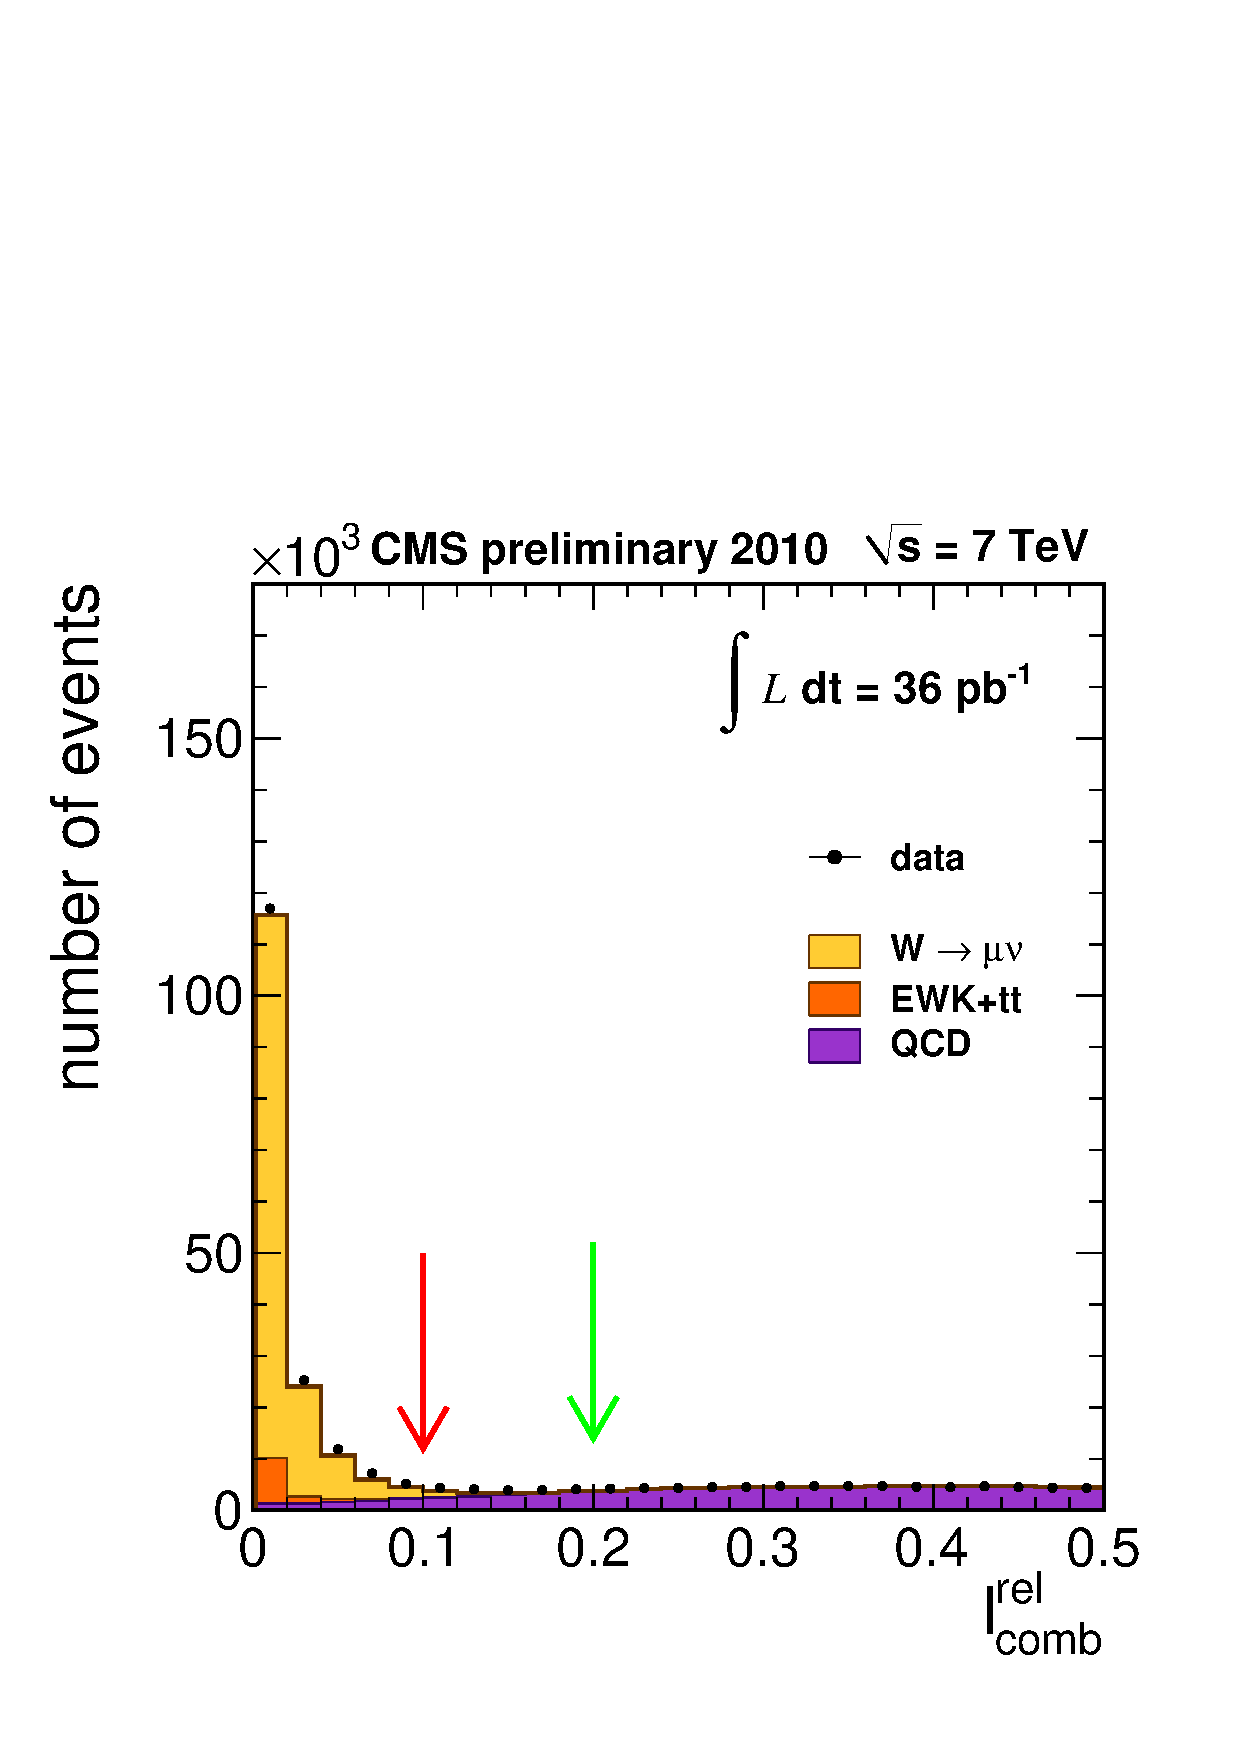
\includegraphics[width=8cm]{figs/Wmunu_isolation.pdf}
    \caption{Isolation distribution of candidates with a good quality muon with $\Pt>25~\GeVc$ and $|\eta|<2.1$.
Dots represent the data and the solid histograms the contribution from the different SM processes, evaluated by MC
and normalized to the theoretical cross sections.}
    \label{figure:Wmunu_iso}}
\end{figure}
166457 events pass the selection described aboved in the data,
97533 (68924) of them with a positive (negative) charged muon.
The acceptance of the selection cuts for $\Wmn$ events within the acceptance
has been estimated with POWHEG MC. The product of acceptance and selection 
efficiency is $\WMIAGEN$ for the whole $\Wo$ sample, and in particular 
$\WMPAGEN$ for $\Wp$ and $\WMMAGEN$ for $\Wm$.
The background fraction is expected to be 12.2\% of the selected sample,
including semi-leptonic decay of quarks mainly from heavy-flavours (5.1\%),
$\Zmm$ events (3.5\%), the electro-weak decays $\Ztt$ (2.7\%) and $\Wtn$ (0.5\%),
$\ttbar$ (0.3\%) and di-boson production
$\Wo\Wo$+$\Wo\Zo$+$\Zo\Zo$ ($0.1$\%). 
Cosmics background, evaluated extrapolating the rate of events with
large impact parameter to the signal region, is found to be negligible ($<0.01\%$).
%(fraction of cosmics background $<10^{-4}$). 

A sum of three contributions of fixed shape is fitted to the observed $\MET$ distribution
with a binned-likelihood fit.
Each of the contributions accounts for a different origin of the
events: W signal, QCD background and EWK background. 
%The distribution of $\MET$ is fit according
%to the following expression:
%\begin{equation}
%N(\MET) = \{ \sigma_W\times [ {\cal A}_W\cdot f_W(\MET) + K \cdot {\cal A}_{EWK}f_{EWK}(\MET)] + {\cal F}_{QCD}f_{QCD}(\MET) \} \times\Lint\,;
%\label{eq:WmnEttemplate}
%\end{equation}
%the W and EWK terms are expressed in terms of the product of cross sections,
%acceptance and selection efficiencies, ${\cal A}_W$ and ${\cal A}_{EWK}$,
%and the $\MET$ probability distribution functions, $f_W$ and $f_{EWK}$.
%$\Zmm$, $\Ztt$ and $\Wtn$ contributions are
%normalized to the $\Wmn$ channel, through their theoretical cross
%section ratio.
%The QCD contribution is described as well in terms of a normalized
%template on $\MET$, $f_{QCD}(\MET)$ and a constant, ${\cal F}_{QCD}$,
%setting the absolute background level.
% ========================== Templates ==================
The signal shape is determined from high statistics MC.
The template is corrected for possible mismodeling in the MC of the $\Et$ scale
and resolution, with information from the recoil of Z events, given the
similarity of W and Z kinematics.
The $\MET$ shape for the other EWK vector boson contributions and $\ttbar$ are
evaluated from MC.
$\MET$ shape for the QCD component is obtained from a high-purity QCD sample, selected
following the same procedure as for the signal, except for the inversion of the
isolation cut: $I^{\textrm{rel}}_{\mathrm{comb}} > 0.2$.
A good agreement between the data template and MC for the not isolated region is observed.
The observed bias of the $MET$ correlated with the isolation is removed applying a correction 
to $\MET$ with varies linearly with $\IRelComb$. We calculate and apply a correction
$\MET^\prime = \MET/(1+\alpha\IRelComb)$, with $\alpha = 0.20\pm 0.08$. 
The same positive correlation is observed in data for the control sample
with $\IRelComb > 0.20$.
We observe that varying the factor $\alpha$ within its uncertainty the template
remains in good agreement with the isolation-inverted template and we account for
the possible corresponding variation of final $\Wo$ yield as systematic uncertainty.

The fitted $\MET$ distributions are presented in
Figure~\ref{figure:Wmunu_exp_fit} (full sample) and Figure~\ref{figure:Wmn_PlusMinus}
 (samples separated by muon charge).
 The fitted individual contributions of the W signal, EWK processes and
 QCD are also shown in the plots. Figures~\ref{figure:Wmunu_exp_fit_mt} and~\ref{figure:Wmn_PlusMinus_mt}
show the $\MT$ distributions for data and fitted signal plus background components.

 \begin{figure}[!ht] {\centering
   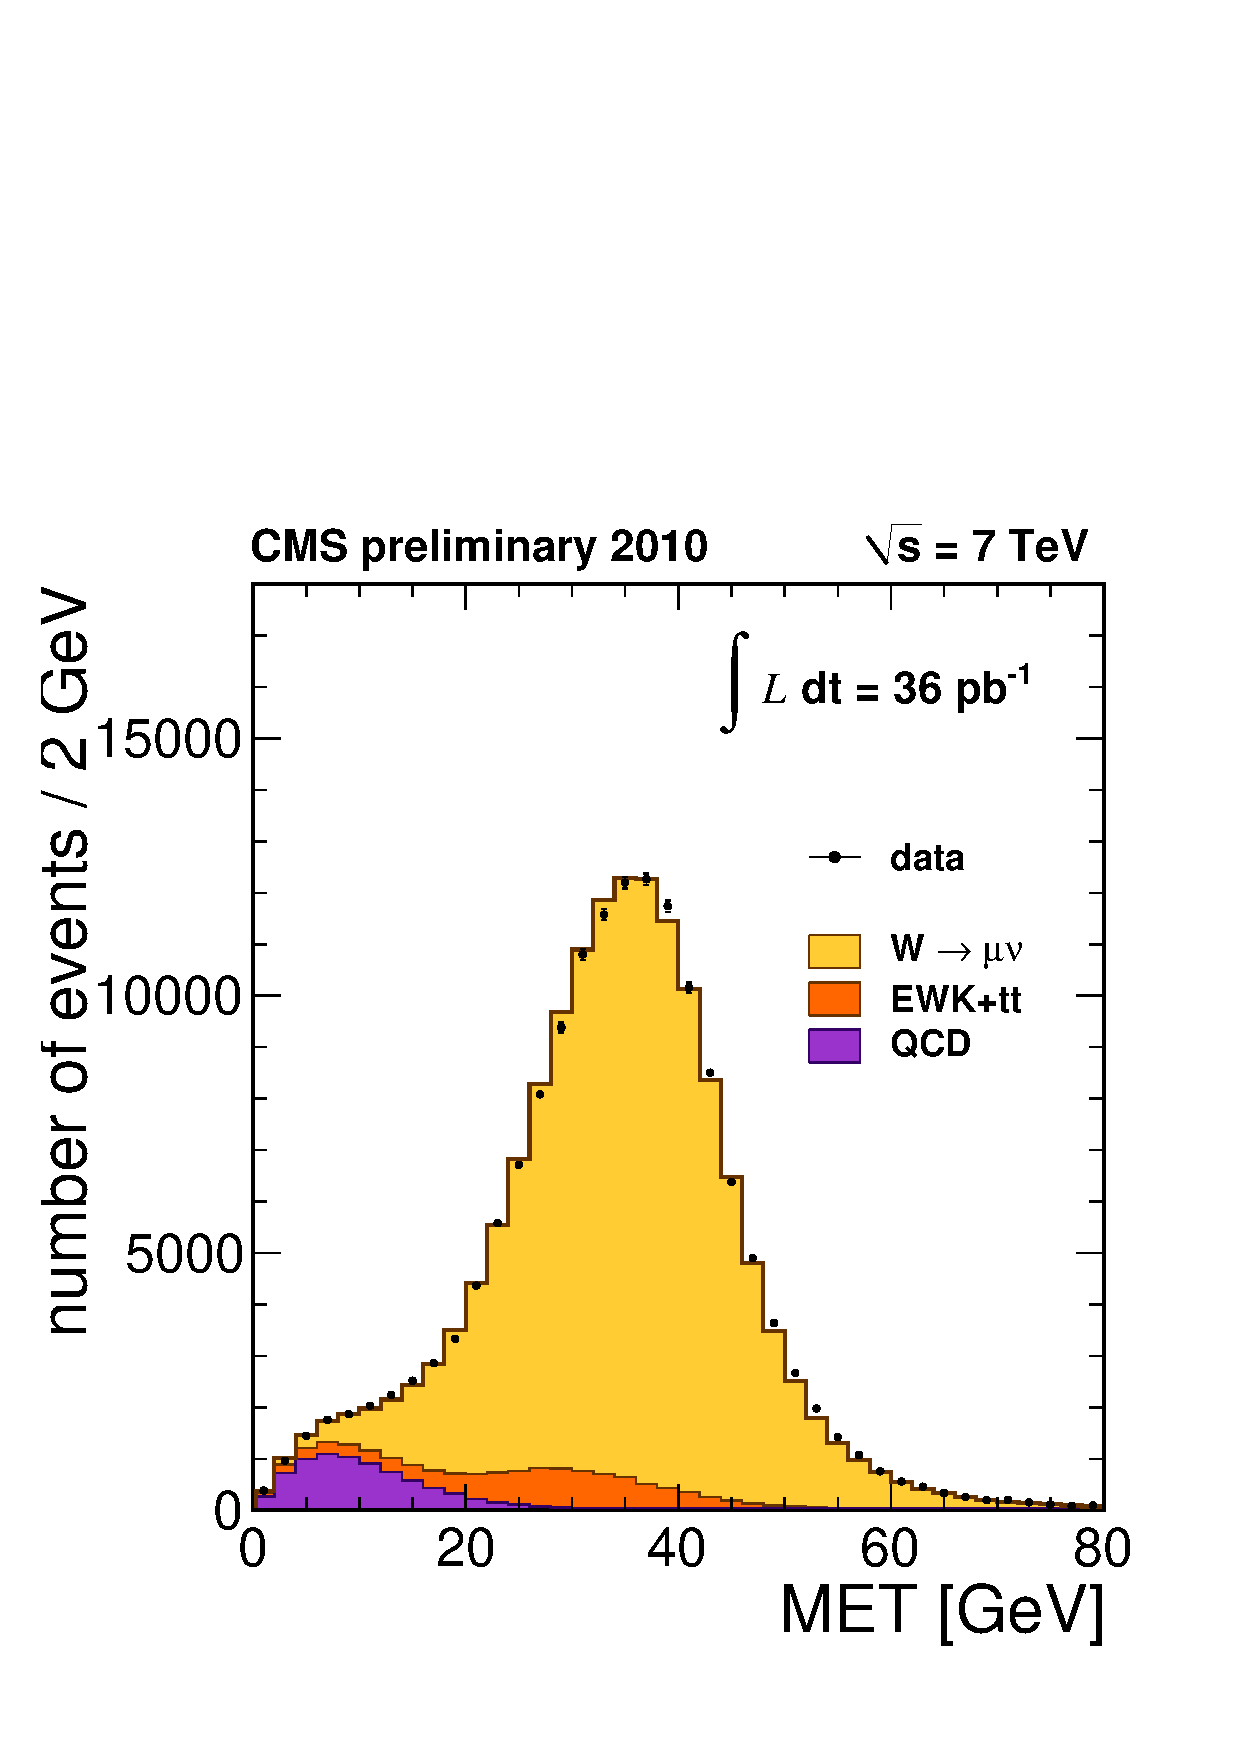
\includegraphics[width=8cm]{figs/Wmn_MET.pdf}
    \caption{Total $\MET$ spectrum (black dots) and fitted contributions from
 the different processes shown stacked, W signal (light yellow histogram), other
 EWK processes (medium orange histogram), and QCD background (dark purple histogram).
 }
     \label{figure:Wmunu_exp_fit}}
 \end{figure}

\begin{figure}[!ht] {\centering
   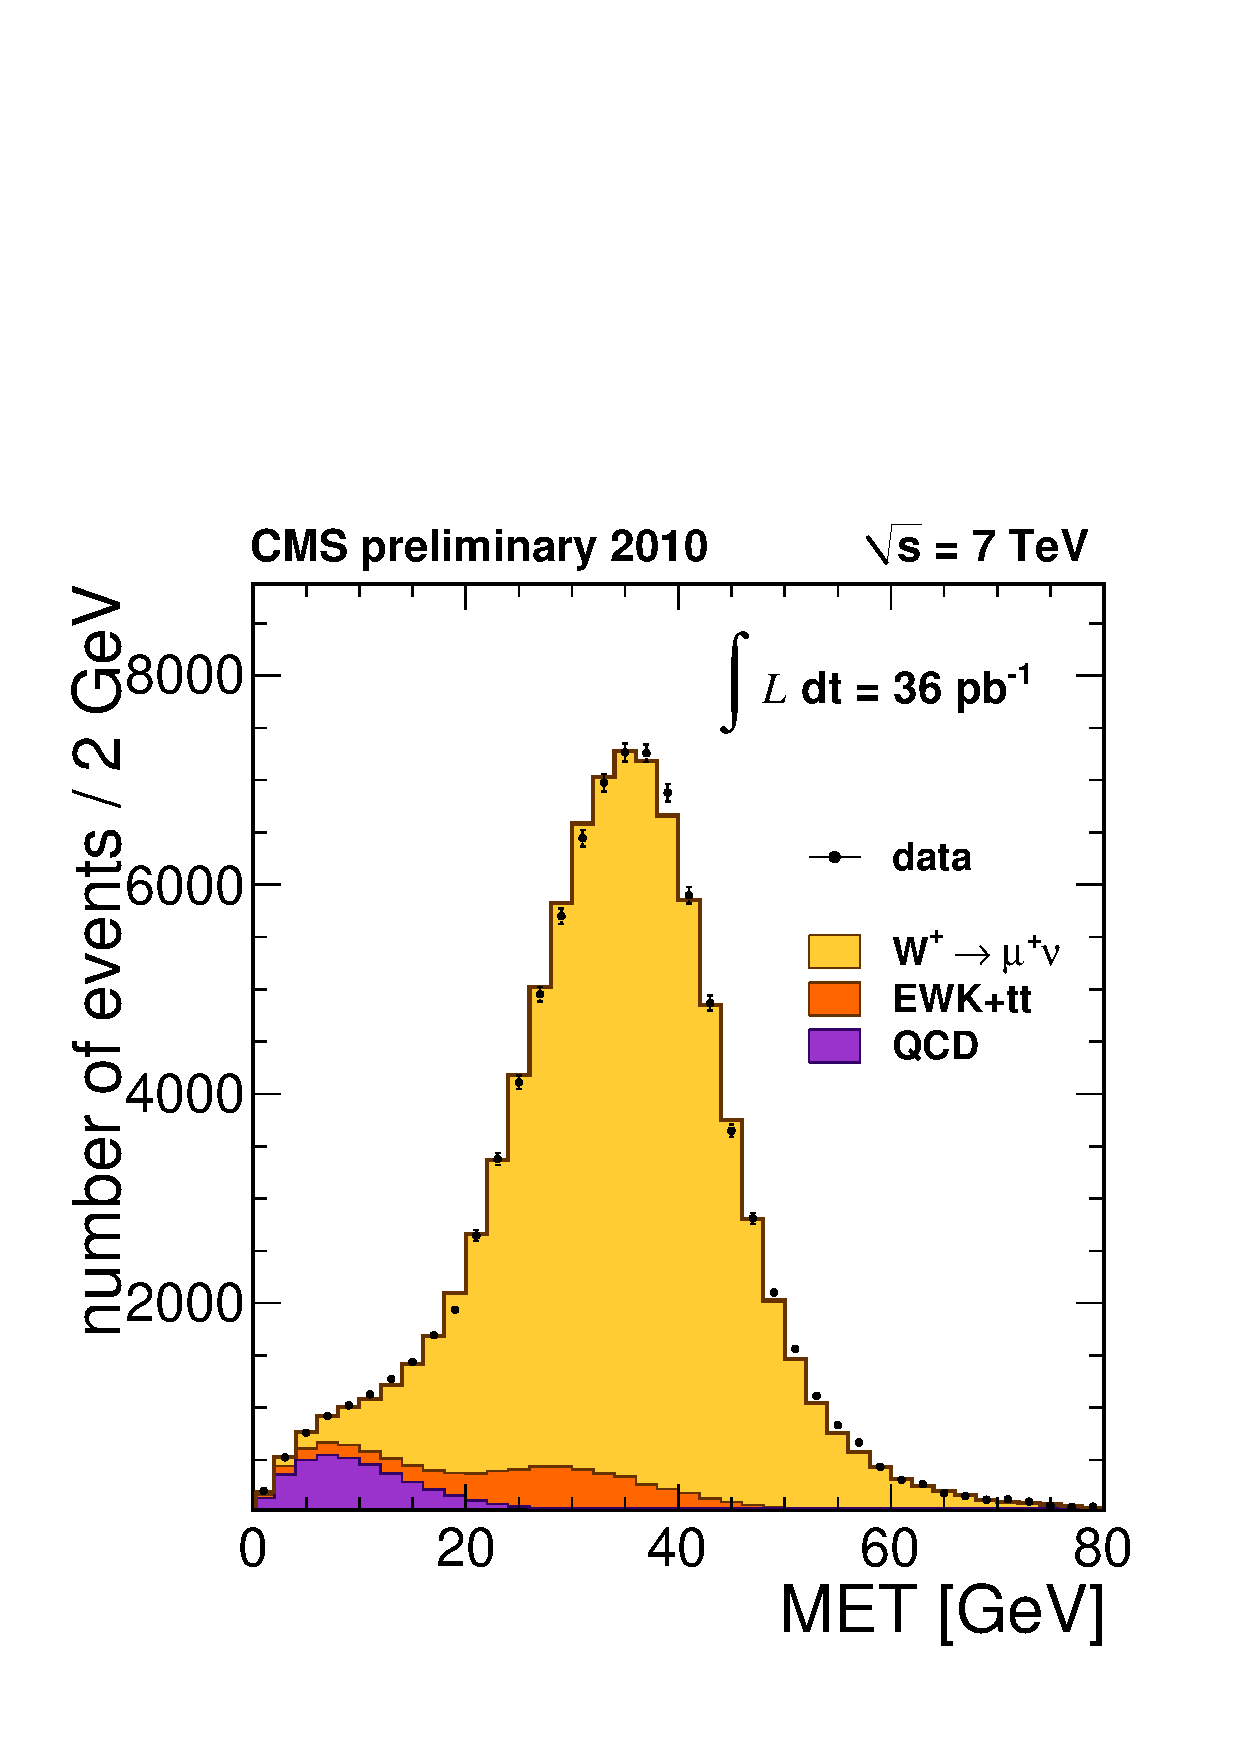
\includegraphics[width=7cm]{figs/Wmn_MET_plus.pdf}
   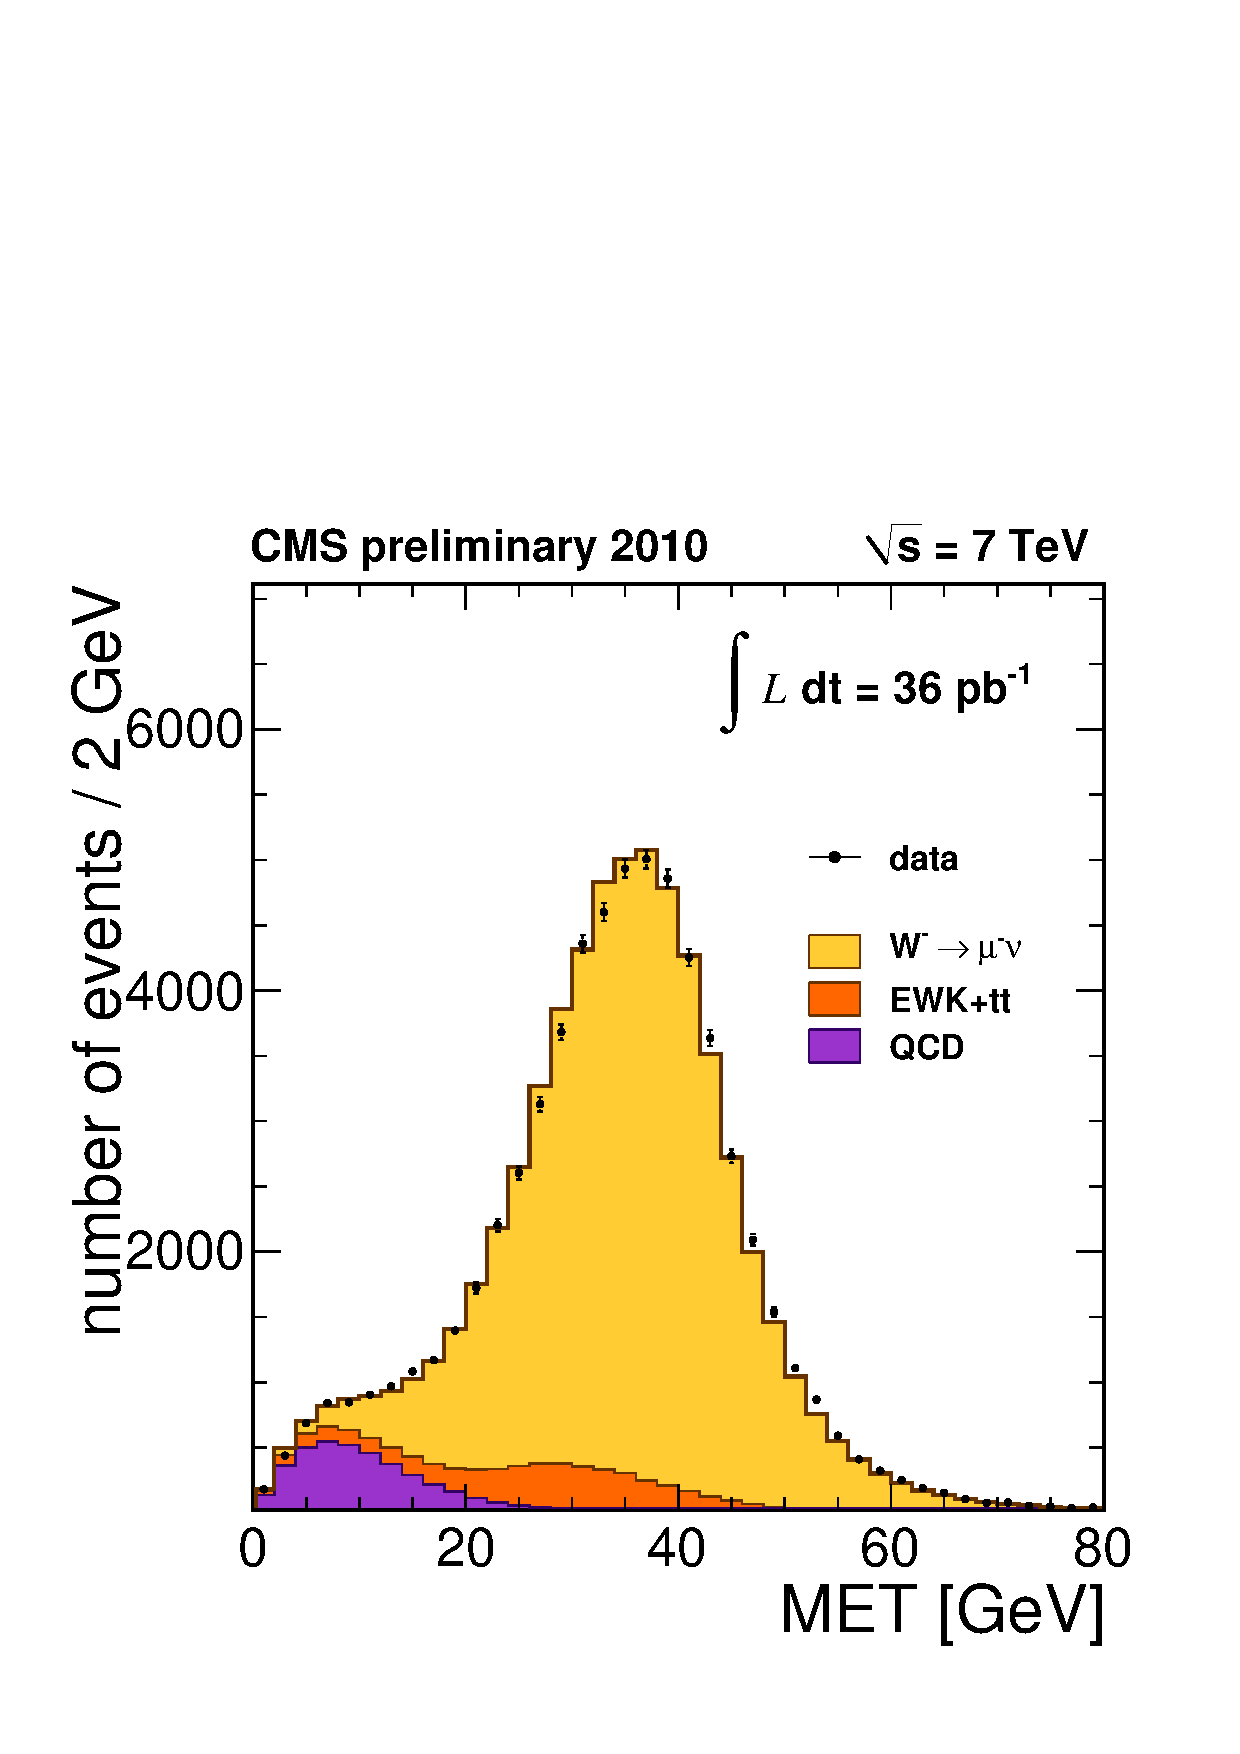
\includegraphics[width=7cm]{figs/Wmn_MET_minus.pdf}
    \caption{
W$^+$ (left plots) and W$^-$ (right plots) experimental distributions (black dots),
together with the fitted contributions from the different processes (shown stacked):
W signal (light yellow histogram), other EWK processes (medium orange histogram),
and QCD background (dark purple histogram).}
    \label{figure:Wmn_PlusMinus}}
\end{figure}

 \begin{figure}[!ht] {\centering
   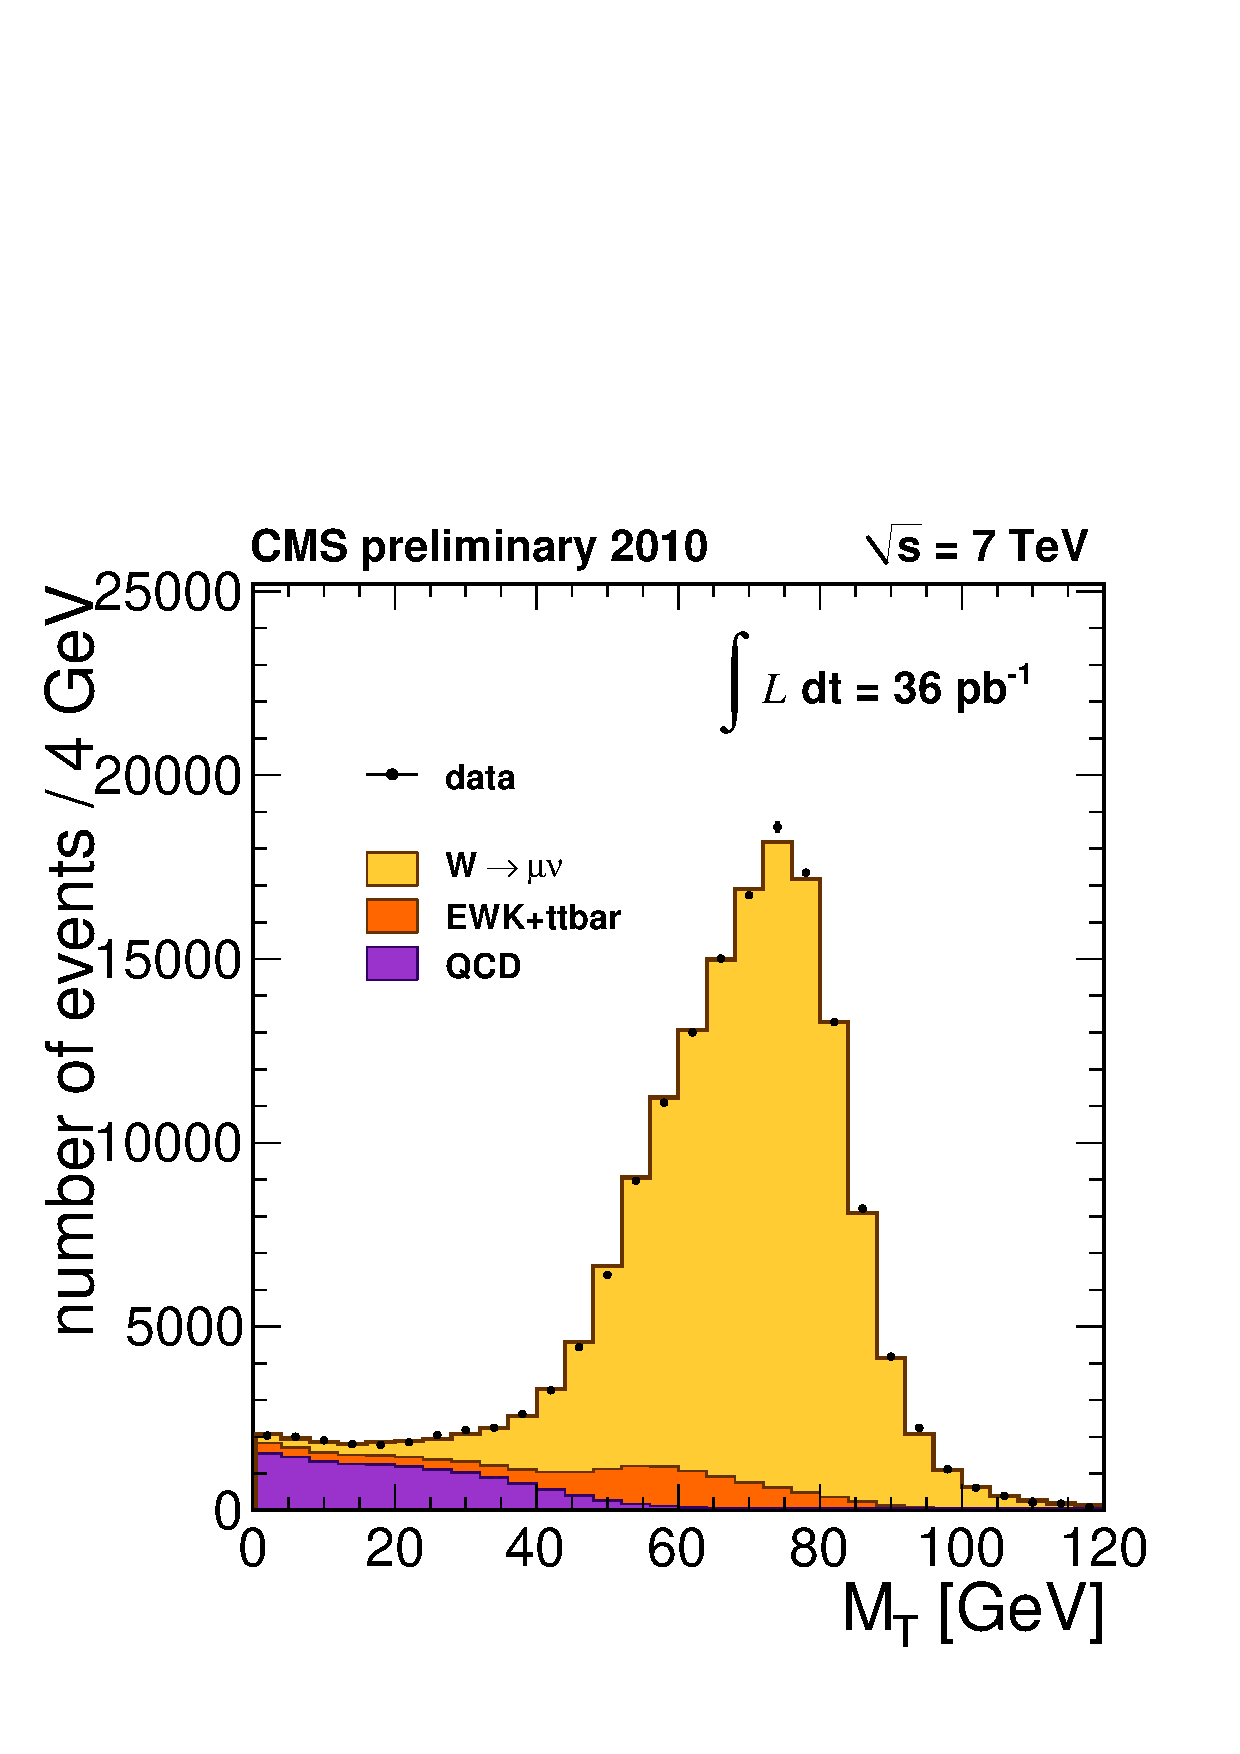
\includegraphics[width=8cm]{figs/Wmn_MT.pdf}
     \caption{Total $\MT$ spectrum (black dots) and fitted contributions from
 the different processes shown stacked, W signal (light yellow histogram), other
 EWK processes (medium orange histogram), and QCD background (dark purple histogram).
 }
     \label{figure:Wmunu_exp_fit_mt}}
 \end{figure}

\begin{figure}[!ht] {\centering
   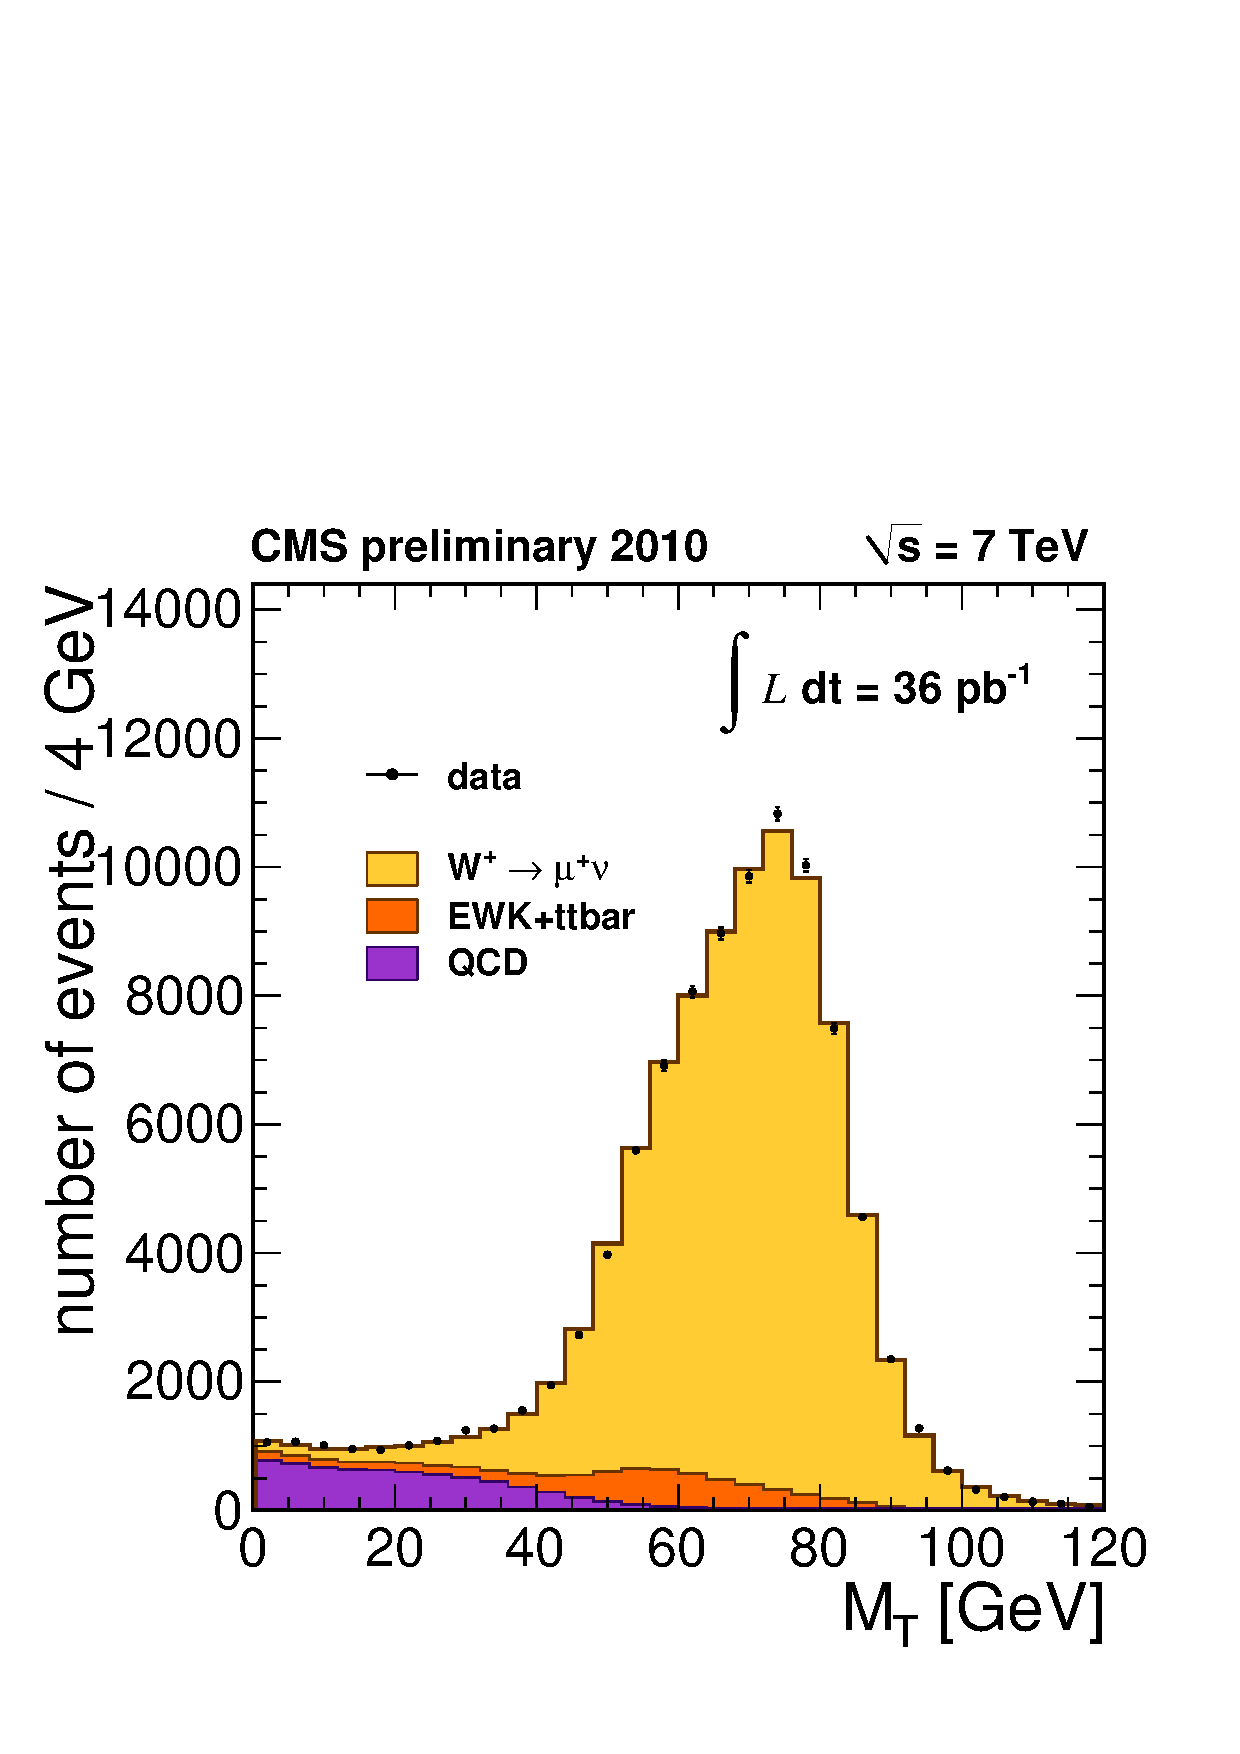
\includegraphics[width=7cm]{figs/Wmn_MT_plus.pdf}
   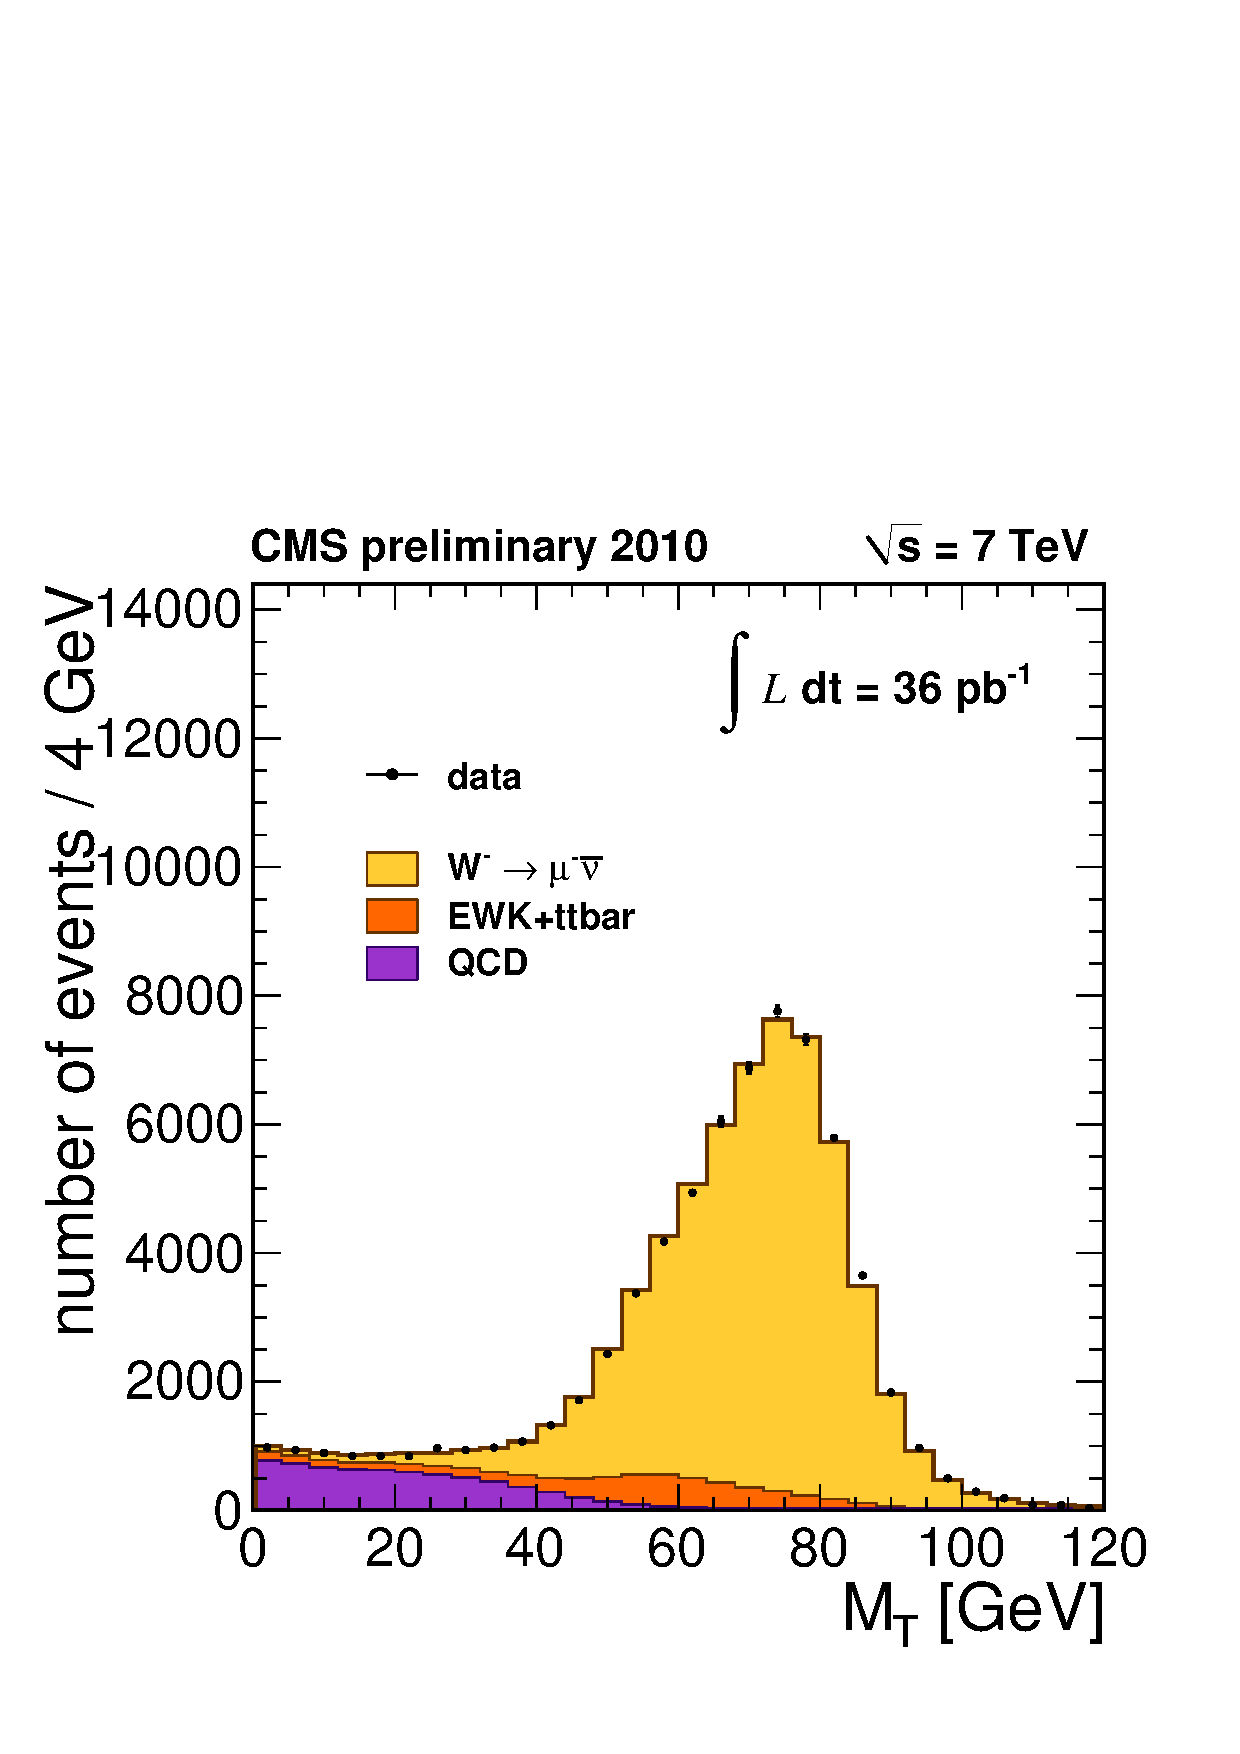
\includegraphics[width=7cm]{figs/Wmn_MT_minus.pdf}
    \caption{
W$^+$ (left plots) and W$^-$ (right plots) $\MT$ distributions (black dots),
together with the fitted contributions from the different processes (shown stacked):
W signal (light yellow histogram), other EWK processes (medium orange histogram),
and QCD background (dark purple histogram).}
    \label{figure:Wmn_PlusMinus_mt}}
\end{figure}

%  The fitted W-parameters are summarized in Tables~\ref{table:Wmunu_tot_xs}
%  for the two choices of fit parameters. The error shown is only statistical.
% \begin{table}[!ht] {\centering
% \begin{tabular}{|c|c|} \hline
%  $\sigma(\mathrm{W})$ (nb)                        & $10.031\pm 0.026$  \\
%  $R = \sigma(\mathrm{W}^+)/\sigma(\mathrm{W}^-)$  & $1.4508\pm 0.0078$ \\ \hline
%  $\sigma(\mathrm{W}^+)$ (nb)                      & $4.093\pm 0.017$    \\
%  $\sigma(\mathrm{W}^+)$ (nb)                      & $5.938\pm 0.020$    \\ \hline
% \end{tabular}
% \caption{Total W production cross section (times the Branching fraction of the W decaying into a
% muon and a neutrino) and ratio between W$^+$ and W$^-$  cross sections from the analysis of
% the $\Lint=36~\pbinv$ data set.}
% \label{table:Wmunu_tot_xs}}
% \end{table}
